%%%%%%%%%%%%%%%%%%%%%%%%%
% Dokumentinformationen %
%%%%%%%%%%%%%%%%%%%%%%%%%
\newcommand{\titleinfo}{Elektrizit\"atslehre 3 - Formelsammlung}
\newcommand{\authorinfo}{Braun \& Co., J.Rast}
\newcommand{\versioninfo}{$Revision: 0 $ - powered by \LaTeX}

%%%%%%%%%%%%%%%%%%%%%%%%%%%%%%%%%%%%%%%%%%%%%
% Standard projektübergreifender Header für
% - Makros 
% - Farben
% - Mathematische Operatoren
%
% DORT NUR ERGÄNZEN, NICHTS LÖSCHEN
%%%%%%%%%%%%%%%%%%%%%%%%%%%%%%%%%%%%%%%%%%%%%
% Genereller Header
\documentclass[10pt,twoside,a4paper,fleqn]{article}
\usepackage[utf8]{inputenc}
\usepackage[left=1cm,right=1cm,top=1cm,bottom=1cm,includeheadfoot]{geometry}
\usepackage[ngerman]{babel,varioref}
\usepackage{multicol}

% Pakete
\usepackage{amssymb,amsmath,fancybox,graphicx,color,lastpage,wrapfig,fancyhdr,hyperref,verbatim}

%%%%%%%%%%%%%%%%%%%%
% Generelle Makros %
%%%%%%%%%%%%%%%%%%%%
\newcommand{\formelbuch}[1]{$_{\textcolor{red}{\mbox{\small{S#1}}}}$}
\newcommand{\verweis}[2]{\small{(siehe auch \ref{#1}, #2 (S. \pageref{#1}))}}
\newcommand{\subsubadd}[1]{\textcolor{black}{\mbox{#1}}}


\newcommand{\skriptsection}[2]{\section{#1 {\tiny Skript S. #2}}}
\newcommand{\skriptsubsection}[2]{\subsection{#1 {\tiny Skript S. #2}}}
\newcommand{\skriptsubsubsection}[2]{\subsubsection{#1 {\tiny Skript S. #2}}}

%%%%%%%%%%
% Farben %
%%%%%%%%%%
\definecolor{black}{rgb}{0,0,0}
\definecolor{red}{rgb}{1,0,0}
\definecolor{white}{rgb}{1,1,1}
\definecolor{grey}{rgb}{0.8,0.8,0.8}
\definecolor{green}{rgb}{0,.8,0.05}
\definecolor{brown}{rgb}{0.603,0,0}
%%%%%%%%%%%%%%%%%%%%%%%%%%%%
% Mathematische Operatoren %
%%%%%%%%%%%%%%%%%%%%%%%%%%%%
\DeclareMathOperator{\sinc}{sinc}
\DeclareMathOperator{\Real}{Re}
\DeclareMathOperator{\Imag}{Im}



% Fouriertransformationen
\unitlength1cm
\newcommand{\FT}
{
\begin{picture}(1,0.5)
\put(0.2,0.1){\circle{0.14}}\put(0.27,0.1){\line(1,0){0.5}}\put(0.77,0.1){\circle*{0.14}}
\end{picture}
}


\newcommand{\IFT}
{
\begin{picture}(1,0.5)
\put(0.2,0.1){\circle*{0.14}}\put(0.27,0.1){\line(1,0){0.45}}\put(0.77,0.1){\circle{0.14}}
\end{picture}
}



%%%%%%%%%%%%%%%%%%%%%%%%%%%%
% Allgemeine Einstellungen %
%%%%%%%%%%%%%%%%%%%%%%%%%%%%
%pdf info
\hypersetup{pdfauthor={\authorinfo},pdftitle={\titleinfo},colorlinks=false}
\author{\authorinfo}
\title{\titleinfo}

%Kopf- und Fusszeile
\pagestyle{fancy}
\fancyhf{}
%Linien oben und unten
\renewcommand{\headrulewidth}{0.5pt} 
\renewcommand{\footrulewidth}{0.5pt}

\fancyhead[L]{\titleinfo{ }\tiny{(\versioninfo)}}
%Kopfzeile rechts bzw. aussen
\fancyhead[R]{Seite \thepage { }von \pageref{LastPage}}
%Fusszeile links bzw. innen
\fancyfoot[L]{\footnotesize{\authorinfo}}
%Fusszeile rechts bzw. ausen
\fancyfoot[R]{\footnotesize{\today}}

% Einrücken verhindern versuchen
\setlength{\parindent}{0pt}

\renewcommand{\arraystretch}{1.5}

% Möglichst keine Ergänzungen hier, sondern in header.tex
\begin{document}
%%%%%%%%%%%%%%%%%%%%%%%%%%%%%%%%%%%%%%%%%%%%%%%%%%%%%%%%%%%%%%%%%%%%%%%%%%%%%%%%%%%%%%%%%%%%%%%%
%%%%%%%%%%%%%%%%%%%%%%%%%%%%%%%%%%%%%%%%%%%%%%%%%%%%%%%%%%%%%%%%%%%%%%%%%%%%%%%%%%%%%%%%%%%%%%%%
\section{Elektrische Felder}
\subsection{Integral-Gesetze der Elektrotechnik}
	\renewcommand{\arraystretch}{2}
	\begin{tabular}{|p{2.5cm}||p{2.7cm}|p{4cm}|p{2.7cm}|p{5cm}|}
	\hline
	& \textbf{Elektr. Feld} & \textbf{Magn. Feld} & \textbf{Strömungsfeld} & \textbf{Bemerkung}\\
	\hline \hline
	Feldgrösse & $\vec{E}$, $\vec{D}$ & $\vec{H}$, $\vec{B}$
	& $\vec{E}$, $\vec{J}$ &\\
	\hline
	Konstante
		& \parbox{2.7cm}{$\varepsilon_0 = 8.854 \cdot 10^{-12}$\\
		{\tiny Dielektrizitätskonstante} \vspace{.1cm}} 
		& \parbox{4cm}{$\mu_0 = 4 \pi \, 10^{-7}$\\ {\tiny Permeabilitätskonstante} \vspace{.1cm}} 
		& \parbox{2.7cm}{$\sigma=\frac{1}{\rho}$ \\ {\tiny Spezifische
		Leitfähigkeit}\vspace{.1cm}} &\\ 
	\hline
	Stoffgleichung & $\vec{D}=\varepsilon_0\varepsilon_r\vec{E}$ & $\vec{B}=\mu_0\mu_r\vec{H}$
	& $\vec{J}=\sigma\vec{E}$ &
	\\
	\hline
	Kraft & $\vec{F_C}=q\vec{E}$ & $\vec{F_L}=q(\vec{v}\times\vec{B})$ &&\\
	\hline
	\parbox{2.5cm}{Fluss\\{\tiny (durch Fläche A)}} & $\Psi_{el}=\int\vec{D}\vec{dA}$ &
	$\Phi_m=\int\vec{B}\vec{dA}$ \textsuperscript{1)}&
	$I=\int\vec{J}\vec{dA}$ & \textsuperscript{1)} bei Spulen:
	$\Psi_m=\sum_i\Phi_i\approx N \Phi$\\
	\hline
	\parbox{2.5cm}{Spannung \\{\tiny (Weg A$\to$B)}} & $U_{AB}=\int\limits_{A}^B
	\vec{E}\vec{ds}$ & $V_{m_{AB}}=\int\limits_{A}^B\vec{H}\vec{ds}$ 
	& $U_{AB}=\int\limits_{A}^B\vec{E}\vec{ds}$ & \\
	\hline
	Schaltelemente & $Q=CU$ & $\Psi_m=LI$, $\Psi_{m21}=M_{21}I_1$
	& $I=GU$, $U=RI$ & $R_m=\frac{1}{\Lambda}$, $R=\frac{1}{G}$\\
	\hline
	\parbox{2.5cm}{Hüllengesetz \\ {\tiny (Quellengleichungen)}}
		& \parbox{2.7cm}{
			\vspace{.1cm}$\oint\vec{D}\vec{dA}=\sum Q_i$ \vspace{.1cm}
			Maxwell IV
			\vspace{.1cm}}
		& \parbox{4cm}{
			\vspace{.1cm}$\oint\vec{B}\vec{dA}=0$
			\textsuperscript{2)} \\
			Maxwell III
			\vspace{.1cm}} 
		& \parbox{2.7cm}{
			$\oint\vec{J}\vec{dA}=0$\\
			Kirchhoff 1}
		& \parbox{5cm}{\textsuperscript{2)} ohne Verschiebungsstrom (käme ggf. noch
		dazu)} \\
	\hline
	Umlaufspannung 
		& \parbox{2.7cm}{
			\vspace{.1cm}
			$\oint\vec{E}\vec{ds}=0-\dot{\Phi}_m$ \\ 
			{\tiny Induktionsgesetz}\\Maxwell II
			\vspace{.1cm}}
		& \parbox{4cm}{
			\vspace{.1cm}
			$\oint\vec{H}\vec{ds}=\theta+\dot{\Psi}_{el}$ \\ 
			{\tiny Vollständiges Durchflutungsgesetz} \\Maxwell I
			\vspace{.1cm}}
		& \parbox{2.7cm}{
			\vspace{.1cm}
			$\oint\vec{E}\vec{ds}=0-\dot{\Phi}$ \\ Kirchhoff 2
			\vspace{.1cm}}
		& \\
	\hline
	\end{tabular}
	\renewcommand{\arraystretch}{1}

\subsection{Einheiten}
\renewcommand{\arraystretch}{1.2}
	\begin{tabular}{|l|l|l|l|l|l|}
	\hline
	$[\varepsilon] = \frac{As}{Vm}$
		& $[D] = \frac{As}{m^2} = \frac{C}{m^2}$
		& $[E] = \frac{V}{m}$
		& $[U] = V$
		& $[\Psi_{el}] = As = C$
		& $[C] = F$ \\
	\hline
	$[\mu] = \frac{H}{m}=\frac{V s}{A m}$
		& $[B] = \frac{Vs}{m^2} = T$
		& $[H] = \frac{A}{m}$
		& $[V_m] = [\Theta] = A$
		& $[\Psi_m] = [\Phi_m] = Wb = Vs$
		& $[L] = \frac{Vs}{A} = H$ \\
	\hline
	$[\sigma] = \frac{S}{m}$
		& $[E] = \frac{V}{m}$
		& $[J] = \frac{A}{m^2} = 10^{-6} \frac{A}{mm^2}$
		& $[U] = V$
		& $[I] = A$
		& $[R] = \Omega$ \\
	\hline
	\end{tabular}
	\renewcommand{\arraystretch}{1}
	
\subsection{Magnetismus}

Magnetische Feldlinien verlaufen ausserhalb eines Magneten vom Nord- zum Südpol
und sind immer geschlossen.\\ 
	\renewcommand{\arraystretch}{2}
	\begin{tabular}[c]{ | p{5cm} | p{8.7cm} | p{4cm} | }
		\hline
		\textbf{Name} & \textbf{Formel} & \textbf{Bemerkung}\\    
		\hline
		\hline
		Lorentzkraft
		& $\vec{F} = Q (\vec{v} \times \vec{B})=I(\vec{l}\times \vec{B}) \hspace{1cm} |\vec{F}| = Q \cdot v \cdot B
		\cdot \sin\alpha$
		&$[\vec{F}]= N$\\
		\hline
		Rechte-Hand-Regel
		& $F$ = Daumen; $v$, $I$ = Zeigefinger; $B$ = Mittelfinger
		& Bei $Q < 0$ wechselt Richtung von B!\\
		\hline
		\parbox{5cm}{Induktionsgesetz\\ \tiny{Allgemeine Form}} &
		$u_i= \mp \dot{\Phi} = \mp \frac{d}{dt} \int \vec{B} \cdot
		\vec{dA}\qquad $ \parbox{3cm}{\tiny{$- \; B,A \Rightarrow$
		Rechtsschraube\\ $+ \; B,A \Rightarrow$
		Linksschraube}} & $[u_i]= V$\\
		& $u_i= \mp \dot{\Psi}\qquad$ , meist $\; u_i = \mp
		N\cdot\dot{\Phi}$ &
		\\
		\hline
		\parbox{5cm}{Induktionsgesetz\\ \tiny{bewegter Leiter im Magnetfeld}} &
		$u_i=\int\vec{E}_i \cdot
		\vec{dl}=-\int(\vec{v}\times \vec{B})\cdot\vec{dl}$ & $[u_i]= V$\\
		& $u_i=v\cdot B \cdot l\qquad$ falls $\vec{v}\perp \vec{B}$ &\\	

		\hline		
		Durchflutungsgesetz
		& $V_m = \oint\vec{H} \cdot \vec{ds} = \int\limits \vec{J}
		\cdot \vec{dA} \vee \underbrace{\sum I_k}_{= N I} = \Theta$
		& $[V_m,\Theta]=A$\\
		\hline
		Magn. Widerstand / Leitwert
		& $R_m = \frac{V_m}{\Phi} = \frac{\Theta}{\Phi} = \frac{l}{\mu A} $ \quad / \quad
		$\Lambda = \frac{1}{R_m}$ & $[R_m]=\frac{A}{Wb}$\;
		/ \;$[\Lambda]=\frac{Wb}{A}$
		\\
		\hline
		Induktivität
		& $L = \frac{\Psi}{I}  \qquad \text{Bei idealer Koppl.: } L = \Lambda N^2 = \frac{N^2}{R_m} $
		& $[L] = \frac{Vs}{A} = H$\\
		\hline
	\end{tabular}
	\renewcommand{\arraystretch}{1}

\subsection{Diverse Formeln bzgl. Magnetismus}
\renewcommand{\arraystretch}{1.1}
\begin{tabular}[c]{|l|l|l|}
\hline
M'feld ausserhalb langen Leiters:
	& M'feld innerhalb geraden, langen Leiters: 
	& Hall-Sonde:\\
$H(r) = \frac{I}{2 \cdot \pi \cdot r}$
	&$H(r) = \frac{I}{2 \pi r} \frac{A_{eingeschlossen}}{A_{total}} = 
	 \frac{I}{2 \pi} \frac{r}{r_a^2}$
	& $U_H = \frac{I \cdot B}{e \cdot n_p \cdot h}$\\
\hline
M'feld der Zylinderspule:
	&M'feld einer Toroidspule:
	&Kraft auf stromführende Leiter:\\
$H(r) = \frac{N \cdot I}{l} \qquad l \gg d$
	& $H_{innen}(r) = \frac{N \cdot I}{2 \cdot \pi \cdot r} \qquad H_{aussen} = 0$
	&$\vec{F_L} = I (\vec{l} \times \vec{B}) \qquad F_L = I \cdot l \cdot B \cdot
	\sin{\alpha}$ \\
\hline
\end{tabular}
\renewcommand{\arraystretch}{1}

\begin{tabular}{llll}
\parbox{4.5cm}{
	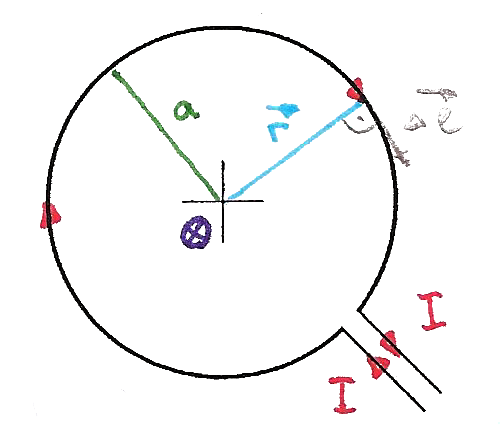
\includegraphics[width=2.7cm]{./bilder/biot1.png} \\
	$H =\frac{I}{D} = \frac{I}{2a}$}
& \parbox{4.5cm}{
	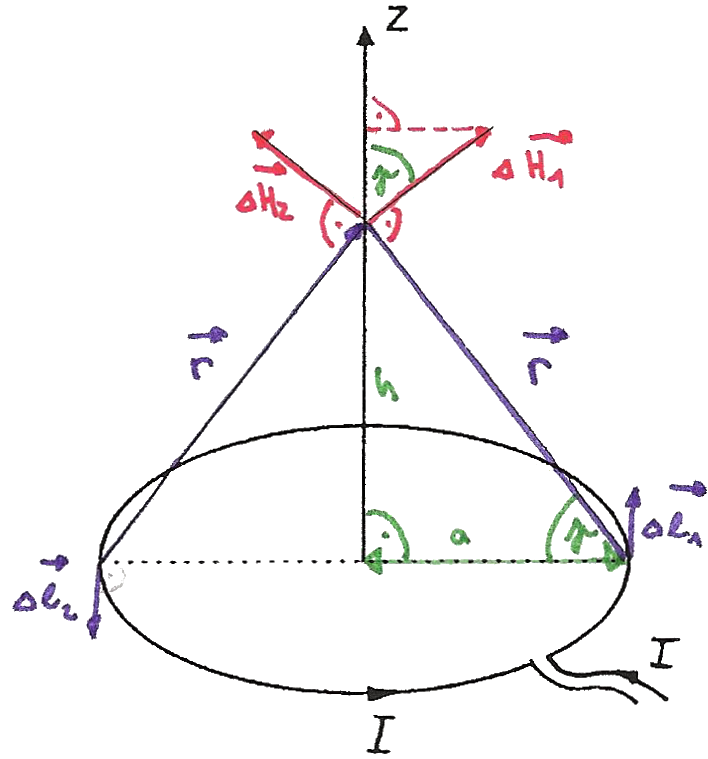
\includegraphics[width=2.7cm]{./bilder/biot2.png} \\
	$H=\frac{I}{2} \cdot \frac{a^2}{\sqrt{a^2+h^2}^3}$}
& \parbox{4.5cm}{
	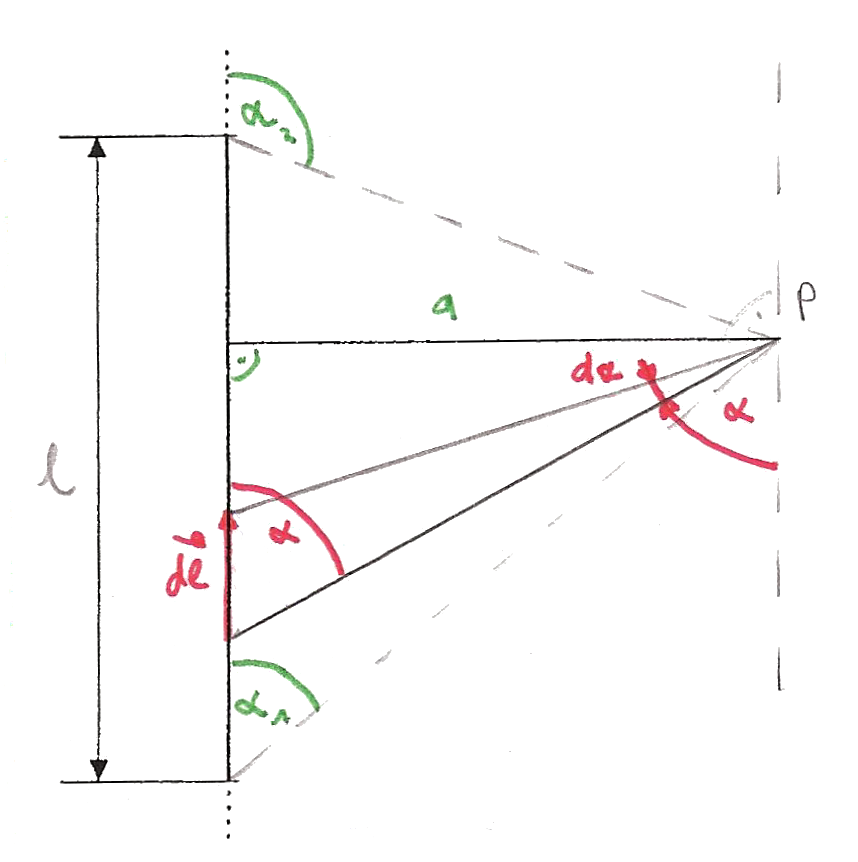
\includegraphics[width=3cm]{./bilder/biot3.png} \\
	$H=\frac{I}{4\pi a}(\cos(\alpha_1)- \cos(\alpha_2))$}
& \parbox{4.5cm}{
	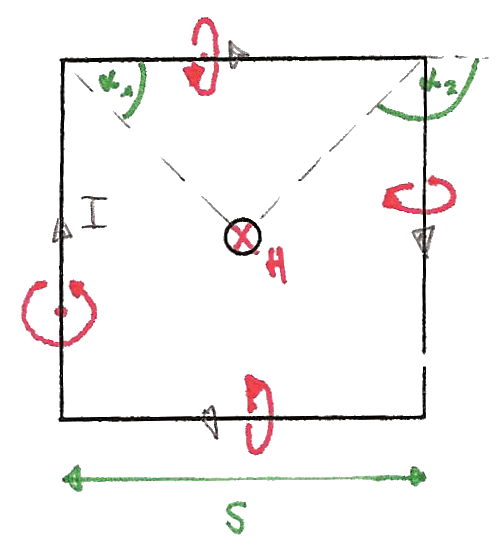
\includegraphics[width=2.7cm]{./bilder/biot4.png} \\
	$H= \frac{I \cdot 2 \sqrt{2}}{\pi \cdot s}$ }
\end{tabular}

\subsection{Zusammenstellung magnetischer Grössen für spezielle
Leiteranordnungen}
\begin{minipage}{9cm}
	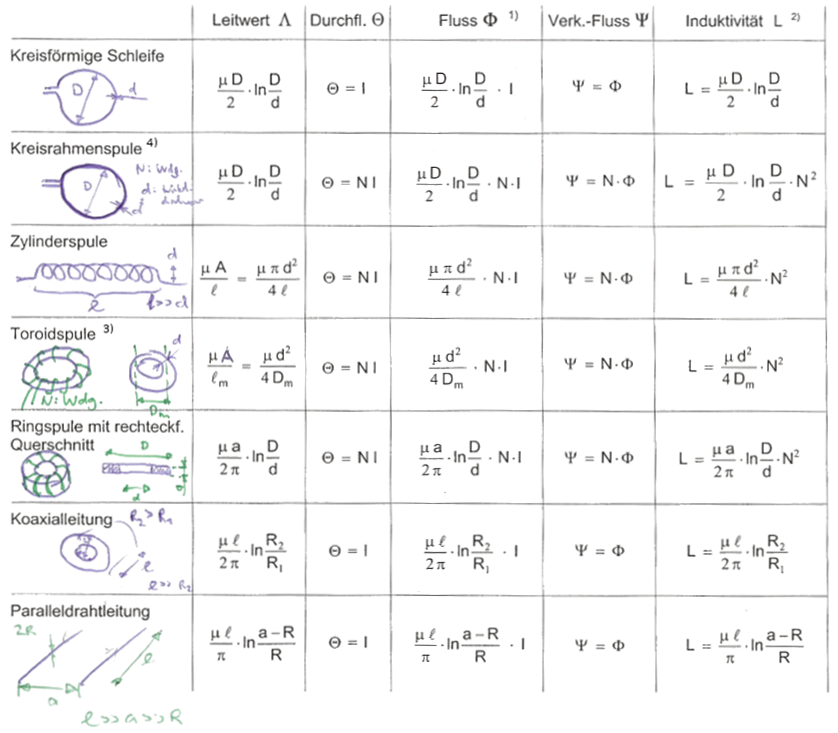
\includegraphics[height=7.5cm]{./bilder/magnetismus_spez_leiteranordnungen.png} 
\end{minipage}
\begin{minipage}[ht]{10cm}
	\textbf{Bemerkungen:}\\
	$^{1)}$ ohne Fluss durch Leiter\\
	$^{2)}$ nur äussere Induktivität\\
	$^{3)}$ $A=\frac{\pi d^2}{4} \qquad l_m \approx \pi D_m$\\
	$^{4)}$ Wickeldurchmesser d in radialer und axialer Richtung $d \ll D$\\
	
	\textbf{Allgemein} gilt:\\
	$\Phi=\Lambda \cdot \Theta$, $\Lambda=\frac{1}{R_m}$\\
	$L=\frac{\Psi}{I}$\\
	$L=\Lambda=\frac{1}{R_m}$, falls $N=1$\\
	$L=\Lambda N^2=\frac{N^2}{R_m}$, falls die $N$-Windungen unter sich ideal
	gekoppelt sind.
\end{minipage}

% trafo im el3 projekt
\subsection{Gegeninduktion, Transformator}

\definecolor{red}{rgb}{1,0,0} % 255,0,0
\definecolor{green}{rgb}{0,.8,0.05} % 0,203,14
\begin{tabular}{ll}
	\parbox{9.5cm}{
 		\textbf{Gegeninduktion} ($M_{\textcolor{red}{X}\textcolor{green}{Y}}; \textcolor{red}{X}$: Wirkung,
 		$\textcolor{green}{Y}$: Ursache)\\
		\begin{tabular}{ll}
  		Gegeninduktivität
  			& $M_{21} = \frac{\Psi_{m21}}{i_1} =$ (Meist $= \frac{N_2
  			\phi_{m21}}{i_1}$)\\ 
  			(wenn $\mu$ = const.) & $M = k \cdot \sqrt{L_1 L_2} = M_{21} = M_{12} $  \\
  			Gegeninduktionsspannung
  			& $u_{21} = \dot{\Psi}_{21} = M_{21} \frac{di_1}{dt}$    
		\end{tabular}}
	& \parbox{8.5cm}{
	  	Durchsetzt das sich ändernde Magnetfeld einer stromdurchflossenen Spule
	  	eine zweite Spule, so wird auch in dieser eine Spannung
	  	(=Gegeninduktionsspannung) induziert.}\\
\parbox{9.5cm}{
		\vspace{.2cm}
  		\textbf{Transformatorgleichungen}\\
		\fbox{$u_1 = L_1 \dfrac{di_1}{dt} \textcolor{red}{+}\textcolor{green}{-}M_{12} \dfrac{di_2}{dt} 
			= L_1 \dfrac{di_1}{dt} \textcolor{red}{-}\textcolor{green}{+}M_{12} \dfrac{di_b}{dt}$} $\qquad$ 
		\fbox{$u_2 = L_2 \dfrac{di_2}{dt}
		\textcolor{red}{+}\textcolor{green}{-} M_{21} \dfrac{d i_1}{dt} 
			= -L_2 \dfrac{di_b}{dt} \textcolor{red}{+}\textcolor{green}{-} M_{21}
			\dfrac{d i_1}{dt}$} 
		\vspace{.2cm}
  			
	  		\textbf{Idealer Trafo}\\ 
	  		\fbox{$"u = \dfrac{u_1}{u_2} = \dfrac{N_1}{N_2} = n$} $\qquad$ (im Leerlauf: $\dfrac{1}{"u} = k \sqrt{\dfrac{L_2}{L_1}}$)
	  		}
  		& \parbox{5cm}{
	  		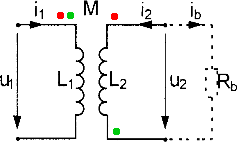
\includegraphics[width=4cm]{../ET3/bilder/trafo-kopplung.png} \\
      		\small{\textcolor{red}{Gleichsinnig} / \textcolor{green}{Gegensinnig}}} \\
	  		
  	\parbox{9.7cm}{
      		\textbf{Verlustbehafteter Trafo}
      		\begin{list}{$\bullet$}{\setlength{\itemsep}{0cm} \setlength{\parsep}{0cm} \setlength{\topsep}{0cm}} 
              \item Primärstrom im Leerlauf: $L_H$
	          	(ideal $L_H \rightarrow \infty)$
	          \item Hysterese- \& Wirbelstromverluste: $R_{Fe}$
	          	(ideal: $R_{Fe}
	          \rightarrow \infty$) 
	          \item Kupferwiderstände: $R_{Cu1}, R_{Cu2}$
	          	(ideal: $R_{Cu}
	          \rightarrow 0$)
	          \item Streufluss (Kopplung): $L_{\sigma1}, L_{\sigma2}$
	          	(ideal: $L_{\sigma} \rightarrow 0$)
            \end{list}
      		}
  		& \parbox{8.8cm}{
	  		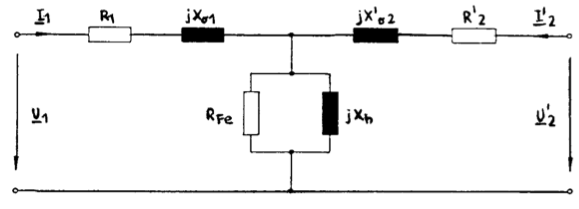
\includegraphics[width=8.8cm]{../ET3/bilder/trafo-verluste.png}}
   	\end{tabular}
\newpage

\section{Wechselstromrechnung}
	\subsection{Allgemein zeitabhängige Grössen}
	\begin{tabular}{|ll|ll|}
    \hline
	\multicolumn{2}{|l}{Arithmetischer Mittelwert, Gleichwert, Linearer MW} 
	    	& \multicolumn{2}{l|}{$X_0 = \overline{X} = X_m = \frac {1} {T} \int\limits_{t_0}^{t_0+T}
	    	x(t)dt$} \\
	\hline
	Quadratischer MW, Leistung 
		& $X^2 = \frac {1} {T} \int\limits_{t_0}^{t_0+T} x^2(t)dt$ 
		& MW $n$. Ordnung
		& $X^n = \frac {1} {T} \int\limits_{t_0}^{t_0+T} x^n(t)dt$ \\
	\hline
	Effektivwert 
		& $X = \sqrt{X^2} = \sqrt{\frac{1}{T} \int\limits ^{t_0+T}_{t_0}{x^2(t)dt}}$
		& Gleichrichtwert 
		& $X_{|m|} = \bar{|X|} = \frac{1}{T} \int\limits_{t_0}^{t_0+T}{|x(t)| dt}$ \\
	\hline
   	\end{tabular}

	\subsection{Begriffe}
		\begin{tabular}{llll}
		$\underline{Z} = R +j X$: 
			& Komplexer Widerstand (Impedanz); 
			& $R$: Wirkwiderstand (Resistanz); 
			& $X$: Blindwiderstand (Reaktanz)\\
		$\underline{Y} = G + j B$: 
			& Komplexer Leitwert (Admittanz); 
			& $G$: Wirkleitwert (Konduktanz); 
			& $B$: Blindleitwert (Suszeptanz)\\
		$\underline{Z}=Z\cdot e^{j\varphi}$ & $Z=\frac{U}{I}=\sqrt{R^2+X^2}$ &
		$\varphi =
		\arctan\left(\frac{\Imag(\underline{Z})}{\Real(\underline{Z})}\right)$&
		$G=\Real(\underline{Y})\neq\frac{1}{R}, \;
		B=\Imag(\underline{Y})\neq\frac{1}{X}$
      	\end{tabular}
	
	\subsection{Schaltelemente bei zeitabhängigen Vorgängen}
	\begin{tabular}{p{1.5cm} p{4.3cm} p{1.5cm} p{4.3cm} p{1.5cm} p{4.3cm}}
   		\multicolumn{2}{l}{\textbf{Ohmscher Widerstand R}}
   			& \multicolumn{2}{l}{\textbf{Kapazitität C}}
   			& \multicolumn{2}{l}{\textbf{Induktivität L}} \\
   		\multicolumn{2}{l}{$u$ und $i$ können sprunghaft ändern}
   			& \multicolumn{2}{l}{$u$ kann nicht sprunghaft ändern}
   			& \multicolumn{2}{l}{$i$ kann nicht sprunghaft ändern} \\
   		\parbox{1.5cm}{
			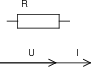
\includegraphics[width=1.5cm]{./bilder/zeigerdiag-r.png}}
			& \parbox{4.3cm}{$u(t) = R i(t)$ \\
				$i(t) = \frac{u(t)}{R}$ \\
				$\underline{Z} = R$}
   			& \parbox{1.5cm}{
				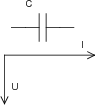
\includegraphics[width=1.5cm]{./bilder/zeigerdiag-c.png}}
			& \parbox{4.3cm}{
				$u(t) = \frac1C \int\limits_0^t i(\tau) d\tau + u(0)$ \\
				$i(t) = C \frac{d u(t)}{dt}$ \\
				$\underline{Z} = \frac{1}{j \omega C} = - \frac{j}{\omega C}$ \\
				$W_C=\frac12 C U_C^2$}
   			& \parbox{1.5cm}{
				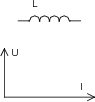
\includegraphics[width=1.5cm]{./bilder/zeigerdiag-l.png}}
			& \parbox{4.3cm}{
				$u(t) = L \frac{di(t)}{dt}$ \\
				$i(t) = \frac1L \int\limits_0^t u(\tau) d\tau + i(0)$ \\
				$\underline{Z} = j \omega L$ \\
				$W_L=\frac12 L I_L^2$}
   	\end{tabular}

	\subsection{Vorgehen bei Schaltvorgängen}
	\fbox{$u(t) =U_E + (U_A - U_E) e^{\frac{-t}{\tau}} \qquad \tau = C R \text{ bzw. }
	\tau =
	 \frac{L}{R} = \frac{\varepsilon}{\sigma} \qquad U_A = \lim\limits_{t
	 \rightarrow 0^+} u(t) \qquad U_E =
	 \lim\limits_{t \rightarrow \infty} u(t)$} $\qquad$ Für Ströme äquivalent
	
	\subsection{Komplexe Darstellung sinusförmiger Vorgänge}
	Momentanwert in $\mathbb{R}$: \fbox{$a(t) = \hat{A} \cos(\omega t + \varphi)$} \qquad
	Momentanwert in $\mathbb{C}$: \fbox{$\underline{a}(t) = \hat{A} e^{j \varphi} e^{j
	\omega t}$} $\qquad$ 
	Amplitude in $\mathbb{C}$: \fbox{$\underline{\hat{A}} = \hat{A} e^{j \varphi}$}\\
	
	Differentiation: $\frac{d}{dt} a(t) = j \omega \underline{\hat{A}}$ $\qquad$ 
	Integration: $\int a(t) dt = \frac{\hat{A}}{j \omega}$
	
	\subsection{Leistungen und Energie}
	\begin{tabular}{ll}
   		\parbox{4cm}{
   			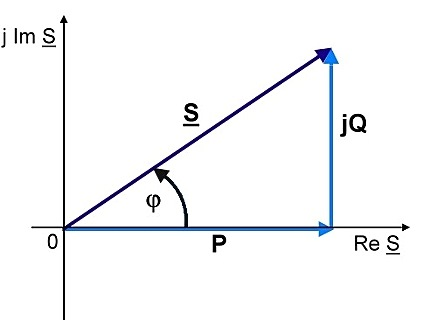
\includegraphics[width=4cm]{./bilder/zeigerdiag-leistungen.png}}
   		& \parbox{14cm}{
			\begin{tabular}{p{3cm}p{5cm}p{5.5cm}}
	      		Momentanleistung
	      			& $p(t) = u(t) i(t)$
	      			\\
				Komplexe Leistung 
					& $ \underline{S} = \underline{U} \cdot \underline{I}^\ast = U\cdot I \cdot
					e^{j(\varphi_u-\varphi_i)}$  & Konjugiert Komplexer Strom! \\
				Wirkleistung
					& $ P = \Real(\underline{S}) = U I \cos(\varphi) $ \\
				Blindleistung 
					& $ Q = \Imag(\underline{S}) = U I \sin(\varphi) $
					& Kapazitiv: $Q < 0$; induktiv: $Q > 0$ \\
				Scheinleistung
					& $ S = | \underline{S} | = U I = \frac{U^2}{R} = I^2 R$ 
					& C: $Q_c=-\omega CU_C^2$, L: $Q_L=\omega LI_L^2$\\
				Leistungsfaktor
					& $\cos \varphi = \frac{P}{S} = \frac{P}{UI}$ \\
				Leistungsanpassung
					& $\underline{Z}_L = \underline{Z}_i^{\ast}; \; P_{max} = \frac{U_q^2}{4
					R_i} = \frac{I_q^2 R_i}{4} $
			\end{tabular}}
   	\end{tabular}

\subsubsection{Blindleistungskompensation}
\begin{tabular}{p{4cm}p{4cm}p{4cm}p{6cm}}
\begin{minipage}{4cm}
    	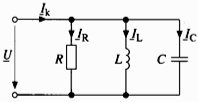
\includegraphics[width=3.5cm]{./bilder/Parallelkompensation.png}
    	\end{minipage}
	& \begin{minipage}{4cm}
    	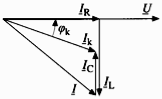
\includegraphics[width=3.5cm]{./bilder/Blindstromkompensation.png}
    	\end{minipage}
	& \begin{minipage}{4cm}
    	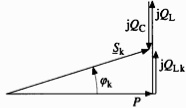
\includegraphics[width=3.5cm]{./bilder/Blindleistungskompensation.png}
    	\end{minipage} 
	& \begin{minipage}{6cm}      
		$$Q_{Lk} = P \cdot \tan{\varphi_k}$$
		$$Q_C = Q_{Lk} - Q_L$$
		$$C = -\frac{Q_C}{\omega U^2}$$
		\end{minipage}
\end{tabular}
\newpage

\subsection{Systematische Netzwerkanalyse}

\subsubsection{Netzwerkgleichungen, Integro-Differentialgleichungen}
Anstelle der Matrizendarstellung werden hier die Netzwerkgleichungen
vollständig ausgeschrieben mit $\int f(t) dt$ und $\frac{d}{dt} f(t)$.	\\ \\

%\subsubsection{Zweigstrommethode / Kreisstrommethode / Maschenstrommethode}
\begin{tabular}{p{9cm}|p{9cm}}
	\begin{minipage}{9cm}
		%\textbf{Zweigstrommethode}\\
		\subsubsection{Zweigstrommethode}		
		\begin{list}{$\bullet$}{\setlength{\itemsep}{0cm} \setlength{\parsep}{0cm} \setlength{\topsep}{0cm}} 
		\item Maschengleichungen enthalten \textbf{Zweigströme} \\
		$\quad\Rightarrow$ Maschen- \& Stromknotengleichungen benötigt\\
		\item kann nicht in Matrizenform dargestellt werden\\  
        \end{list} 
		\hrule
		\vspace{0.2cm}
		%\textbf{Kreis- oder Maschenstrommethode} (s. Bilder rechts)\\
		\subsubsection{Kreis- oder Maschenstrommethode} (s. Bilder rechts)\\
		\begin{list}{$\bullet$}{\setlength{\itemsep}{0cm} \setlength{\parsep}{0cm} \setlength{\topsep}{0cm}} 
			\item Maschengleichungen enthalten \textbf{Maschenströme}\\
			$\quad\Rightarrow$ nur Maschengleichungen benötigt\\
			\item Kann in Matrizenform dargestellt werden\\
		    \item \textcolor{brown}{Baum} verbindet alle \textcolor{red}{Knoten}, ist
		    aber nie geschlossen\\
		    \item Aufzustellende \textcolor{green}{Maschen} bestehen immer aus beliebig
		    vielen \textcolor{brown}{Ästen} (Zweige vom Baum) und \textbf{einer Sehne}
	    \end{list}	
    \end{minipage} &
	\begin{minipage}{9cm}
    		\underline{Bild 1}\\
    		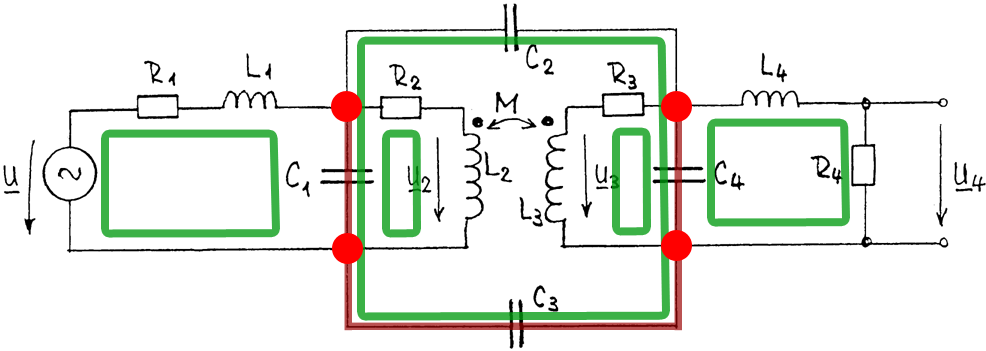
\includegraphics[height=3cm]{./bilder/netzwerkanalyse-kreisstrom2.png}\\
			\underline{Bild 2}\\
			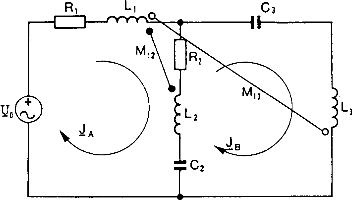
\includegraphics[height=3.5cm]{./bilder/netzwerkanalyse-maschenstrom.png}\\
    		\\
    		\\
    		\hrule
    \end{minipage}\\
\end{tabular} \\
\\ \\
\textbf{Matrix der Maschenstrommethode (Bild 2)}
$$\left[ \begin{array}{cc}
        R_1+R_2 +j \omega L_1 + \frac{1}{j \omega C_2} + j \omega L_2 - j 2
        \omega M_{12} 
    & -(R_2 + j \omega L_2 + \frac{1}{j \omega C_2} - j \omega M_{12} -
        j \omega M_{13}) \\
    -(R_2 + j \omega L_2 + \frac{1}{j \omega C_2} - j \omega M_{12} - j
        \omega M_{13})
    & R_2 + j \omega L_2 + j \omega L_3 + \frac{1}{j \omega C_2} +
        \frac{1}{j \omega C_3}
\end{array}\right] \cdot
\left[ \begin{array}{cc}
     \underline{J}_A \\ \underline{J}_B
     \end{array}\right] =
\left[ \begin{array}{cc}
     U_0 \\ 0
     \end{array}\right]$$
$$\textbf{Allgemein: }\left[ \begin{array}{cc}
       \text{Impedanzen $\underline{Z}$} \\
       \text{symmetrisch zur Diagonalen}
%       \text{Diagonale positiv, sonst negativ}
       \end{array}\right] \cdot \left[ \begin{array}{cc}
     \text{Maschenströme $\underline{J}$}
     \end{array}\right] =
\left[ \begin{array}{cc}
     \text{Spannungsquellen $\underline{U}$} \\
    \text{Gegenrichtung positiv, sonst negativ}
     \end{array}\right]$$\\

\subsubsection{Gekoppelte Spulen}
\begin{center}
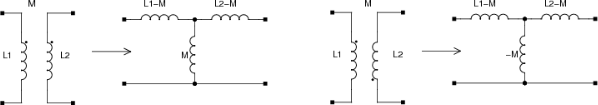
\includegraphics[width=14cm]{./bilder/netzwerkanalyse-kopplung-spulen.png}
\end{center}

\textbf{Vorzeichen der Gegeninduktivität}: 
Fliesst der ``fremde`` (induzierende) Strom bei der \textbf{Markierung hinein}, so hat er dieselbe
Wirkung als wenn er bei der gekoppelten Spule in die \textbf{Markierung
hineinfliessen würde}! 

\newpage
\subsubsection{Knotenpotentialmethode oder Trennbündelmethode}
\begin{tabular}{ll}
\parbox{6cm}{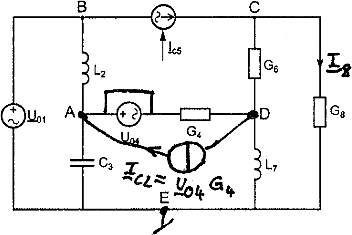
\includegraphics[width=6cm]{./bilder/netzwerkanalyse-knotenpotential.png}
	}
	& \parbox{12cm}{
	Gegeben: $\underline{I}_{C5} = k \underline{I}_8$
	\begin{itemize}
      \item Knoten B hat keine Gleichung, da $E_B = \underline{U}_{01}$
      \item Rechnung nur mit \textit{Admittanzen} (Leitwerten) $\underline{Y}
      = \frac{1}{\underline{Z}} = G + jB$
      \item Schema mit (idealen) \textit{Stromquellen}
    \end{itemize}
$$\begin{bmatrix}
    G_4 + \frac{1}{j \omega L_2} + j \omega C_3 & 0 & -G_4 \\
    0 & G_6 + G_8 - \underbrace{k G_8}_{\underline{I}_{C5}} & -G_6 \\
    -G_4 & -G_6 & \frac{1}{j \omega L_7} + G_4 + G_6   
	\end{bmatrix} \cdot
\begin{bmatrix}
    \underline{E}_A \\ \underline{E}_C \\ \underline{E}_D
    \end{bmatrix} =
\begin{bmatrix}
    \underline{U}_{04} G_4 + \frac{\underline{U}_{01} }{j \omega L_2}\\ 
    0 \\
    -\underline{U}_{04} G_4 \end{bmatrix}$$    
	}
\end{tabular}

$$\textbf{Allgemein: }\left[ \begin{array}{cc}
       \text{Admittanzen $\underline{Y}$} \\
       \text{symmetrisch zur Diagonalen}
%       \text{Diagonale positiv, sonst negativ}
       \end{array}\right] \cdot \left[ \begin{array}{cc}
     \text{Knotenpotentiale $\underline{E}$}
     \end{array}\right] =
\left[ \begin{array}{cc}
     \text{Stromquellen $\underline{J}$} \\
    \text{Hineinfliessen positiv, sonst negativ}
     \end{array}\right]$$

\subsubsection{Aspekte zur Wahl der Methode}
\begin{tabular}{lll}
\multicolumn{3}{l}{\textit{Art der gegebenen Quellen}}\\
&Kreisstrommethode: &Spannungsquellen\\
&Knotenpotentialmethode: &Stromquellen\\
\multicolumn{3}{l}{\textit{Anzahl Gleichungen}}\\ &Kreisstrommethode: &$z-k+1-$ Anzahl idealer Stromquellen\\
&Knotenpotentialmethode: &$k-1-$ Anzahl idealer Spannungsquellen\\
\multicolumn{3}{l}{\textit{Spezialitäten}}\\
&Kreisstrommethode: &Gegeninduktivitäten\\
&Knotenpotentialmethode: &Gesteuerte Stromquellen\\
\multicolumn{3}{l}{\textit{Gesuchte Grössen}}\\
&Kreisstrommethode: &(Sehnen-) Ströme\\
&Knotenpotentialmethode: &(Knoten-) Spannungen
\end{tabular}

\subsection{Stern-Dreieck-Umwandlung}% \formelbuch{18}}
	%\begin{figure}
	  \begin{minipage}[lt]{7.5 cm}
	    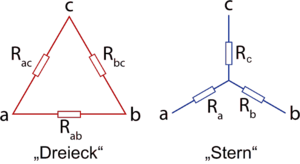
\includegraphics[width=6cm]{./bilder/stern-dreieck.png} 
	  \end{minipage}
	  \begin{minipage}[rt]{9.35 cm} %BASTEL!!
      \renewcommand{\arraystretch}{2}
	  \begin{tabular}{ll}
	Umwandlung $\triangle \rightarrow Y$: 
		&$Z_{c} = \dfrac{Z_{ac} Z_{bc}}{Z_{ab}+Z_{bc}+Z_{ac}}$\\
	Umwandlung $Y \rightarrow \triangle$: 
		&$Y_{ac}=\dfrac{Y_{a} Y_{c}}{Y_{a}+Y_{b}+Y_{c}}$\\
	Bei gleichen Widerständen:
	&$R_Y = \frac{R_\triangle}{3}$ \\
	Bei gleichen Kapazitäten:
	&$C_Y = C_\triangle \cdot 3 $ \\
	Bei gleichen Induktivitäten:
	&$L_Y = \frac{L_\triangle}{3}$
	  \end{tabular}
      \renewcommand{\arraystretch}{1}
	  \end{minipage}

\newpage
\subsection{Impedanz-Transformationen}
Werden gebraucht, wenn Bauteile verschiedene Werte haben können. Bspw. wird in
einer Schaltung eine Kapazität oder eine Induktion variiert.\\
%Immer zuerst die einfachere Variante (Serieschaltung: \underline{Z},
%Parallelschaultung: \underline{Y}) darstellen und daraus die andere Ortskurve herleiten. \\
Bei der Umwandlung von \underline{Z} nach \underline{Y} und umgekehrt handelt es sich um die
\textbf{komplexe Kehrwertfunktion}: 
\begin{itemize}
  \item $\underline{Y} = \frac{1}{\underline{Z}} 
  ( arg(\underline{Z}) = -arg(\underline{Y}),  
  |\underline{Y}| = \frac{1}{| \underline{Z} |}) \qquad$
  (Unendlich ferner Punkt wird in den Ursprung abgebildet und umgekehrt)
  \item Verläuft die OK von \underline{Z} oberhalb der Re-Achse, so verläuft die OK von
  \underline{Y} unterhalb der Re-Achse und umgekehrt.
\end{itemize} 
\textbf{Konstruktion} der kreisförmigen Ortskurve:
\begin{enumerate}
  \item Andere Orstkurve (komplexer Kehrwert) als Gerade darstellen. (Dient als Orientierungshilfe
  und zur Überprüfung)
  \item Extremalwerte berechnen und als Punkte $P_1, P_2$ darstellen. 
	($P_1 = \underline{Z}_0 = \lim\limits_{R \rightarrow 0}\underline{Z}, \quad
	  P_2 = \underline{Z}_\infty = \lim\limits_{R \rightarrow \infty}\underline{Z} $)
  \item Mittelsenkrechte von $P_1, P_2$ konstruieren, deren Schnittpunkt mit Re- \textbf{oder}
  Im-Achse den Kreismittelpunkt $M$ ergibt. \\
  Mittels Betrachtung des Anfangswinkels ($\varphi_{Z_0} = - \varphi_{Y_0}$  oder
  $\varphi_{Z_\infty} = - \varphi_{Y_\infty}$) kann die Anfangsrichtung des Kreises in
  der Nähe des Ursprungs bestimmt werden und der ''falsche'' Mittelpunkt ($M_{Re}$ oder $M_{Im}$)
  ausgeschlossen werden.
  \item Ortskurve (Kreis mit Mittelpunkt $M$, schneidet $P_2$ und $P_1$) konstruieren
\end{enumerate}

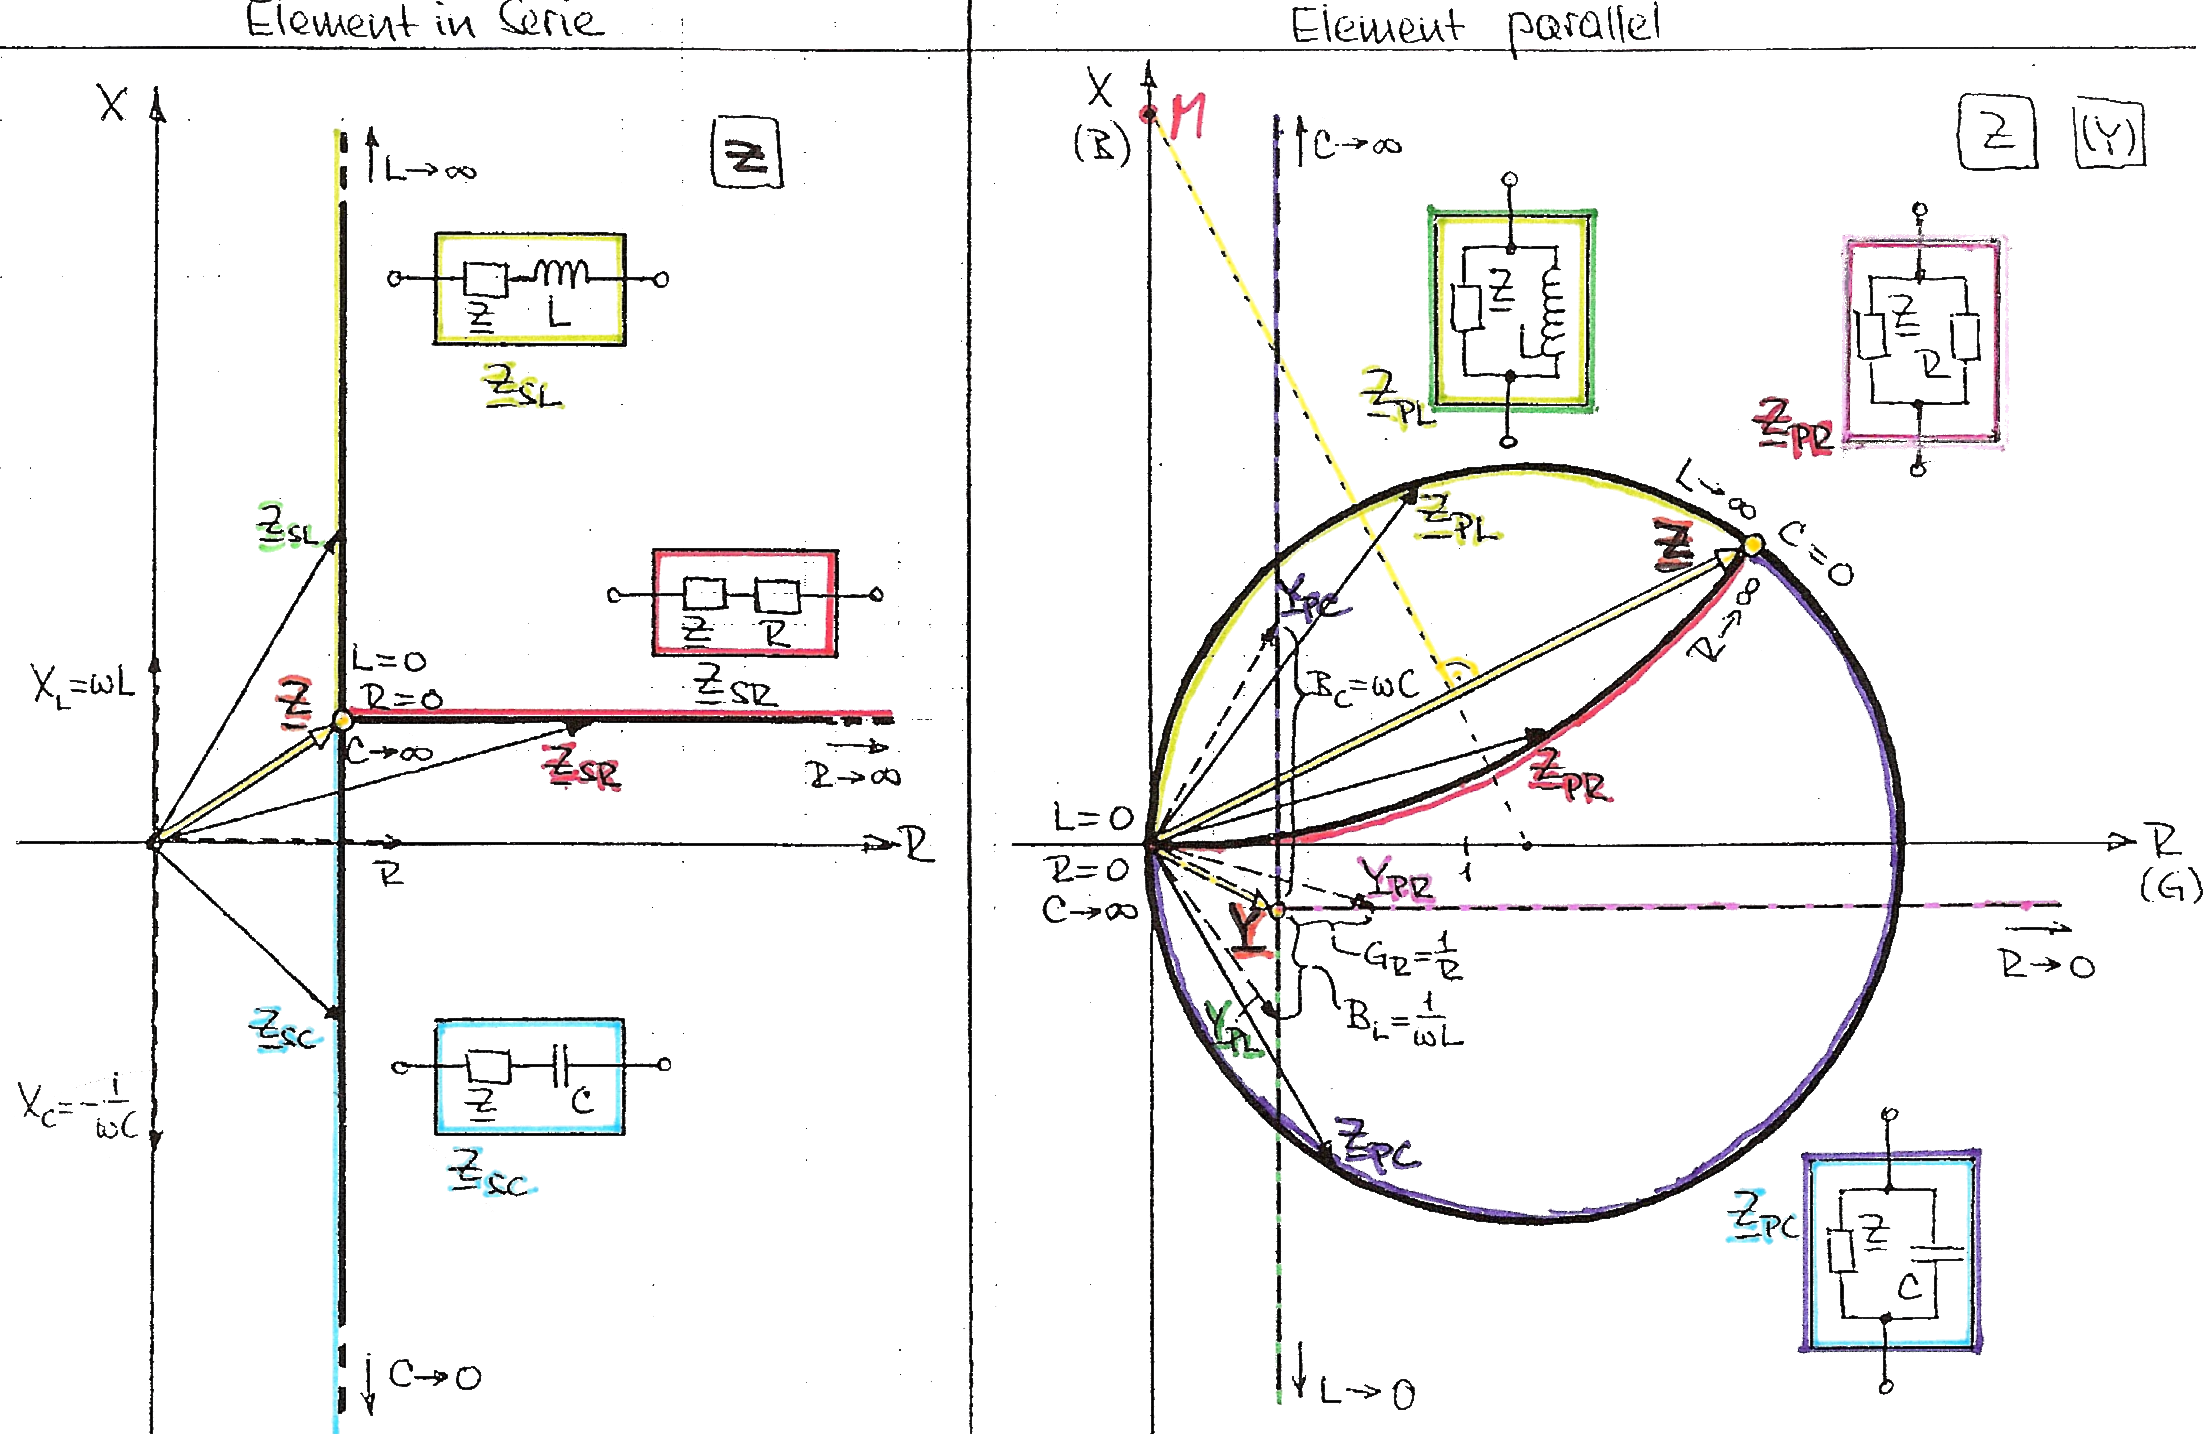
\includegraphics[width=18cm]{./bilder/impedanztrafo.png}

\section{Mathematische Formeln}
\begin{tabular}{lll}
	& \parbox{9.5cm}{
		\textbf{Cosinussatz} \\
		$$c^2 = a^2 + b^2 - 2 \cdot a \cdot b \cdot \cos \gamma$$\\
		\textbf{Sinussatz} \\
		$$\frac{a}{\sin \alpha} = \frac{b}{\sin \beta} = \frac{c}{\sin \gamma} = 2r =
		\frac{u}{\pi}$$}
	& \parbox{8cm}{
		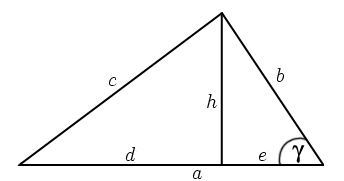
\includegraphics[width=6cm]{./bilder/cosinussatz.png}}

\end{tabular}

\end{document}


